%                                                                 aa.dem
% AA vers. 8.2, LaTeX class for Astronomy & Astrophysics
% demonstration file
%                                                       (c) EDP Sciences
%-----------------------------------------------------------------------
%
%\documentclass[referee]{aa} % for a referee version
%\documentclass[onecolumn]{aa} % for a paper on 1 column
%\documentclass[longauth]{aa} % for the long lists of affiliations
%\documentclass[rnote]{aa} % for the research notes
%\documentclass[letter]{aa} % for the letters
%\documentclass[bibyear]{aa} % if the references are not structured
% according to the author-year natbib style

%
\documentclass{aa}

%
\usepackage{graphicx}
%%%%%%%%%%%%%%%%%%%%%%%%%%%%%%%%%%%%%%%%
\usepackage{txfonts}
%%%%%%%%%%%%%%%%%%%%%%%%%%%%%%%%%%%%%%%%
\usepackage{hyperref}
\hypersetup{pdfborder=0 0 0, colorlinks=true, linkcolor=black, urlcolor=blue,
citecolor=black}
% To add links in your PDF file, use the package "hyperref"
% with options according to your LaTeX or PDFLaTeX drivers.
%
\renewcommand{\thefootnote}{\fnsymbol{footnote}}
\newcommand{\Sun}[0]{\ensuremath{_{\odot}}}
\newcommand{\mytilde}{\raise.17ex\hbox{$\scriptstyle\mathtt{\sim}$}}
\begin{document}


   \title{Star Cluster and Giant Molecular Cloud Interaction with AMUSE}

   \subtitle{Computational Astrophysics (CA) assignment three}

   \author{T. Halbesma (1603221)
          \inst{1}
          \and
          S. Sultan (1617451)\inst{2}
          }

   \institute{Anton Pannekoek Instituut (API), University of Amsterdam,
              Science Park 904, 1098 XH Amsterdam
              \email{timo.halbesma@student.uva.nl}
         \and
             Informatics Institute, Section Computational Science, University of Amsterdam,
             Science Park 904, 1098 XH Amsterdam
             \email{shabaz.sultan@student.uva.nl}
             }

   %\date{Received September 15, 1996; accepted March 16, 1997}

% \abstract{}{}{}{}{}
% 5 {} token are mandatory

  \abstract
  % context heading (optional)
  % {} leave it empty if necessary
   {}
  % aims heading (mandatory)
   {}
  % methods heading (mandatory)
   {}
  % results heading (mandatory)
   {}
  % conclusions heading (optional), leave it empty if necessary
   {}

   \keywords{Hydrodynamics --
                AMUSE --
               }

   \maketitle
%
%________________________________________________________________

\section{Introduction}
In this report, the authors have used the Astrophysical Multipurpose Software Environment, in short AMUSE \citep{2009NewA...14..369P, 2013CoPhC.183..456P, 2013A&A...557A..84P}. Firstly, a stellar cluster is created where the gravitational interactions between the stars are calculated by the N-Body algorithm developed by Barnes and Hut, the BHTree \cite{1986Natur.324..446B}. In addition, we set up a giant molecular cloud (GMC) using Smoothed Particle Hydrodynamics (SPH) to simulate the gas and dust in the cloud. In particular, we use the TreeSPH hydrodynamics code `FI' \citep{1989ApJS...70..419H, 1997A&A...325..972G, 2004A&A...422...55P, 2005PhDT........17P}. Choosing an SPH hydrodynamics code enables us to study the gravity in the system as if two N-Body systems are interacting because the gas is split up in different regions represented by SPH particles. The gravity code can act on these particles. In AMUSE two (or more) gravity systems can be coupled using the Bridge interface. The Bridge interface, thus, is used to couple the GMC and the stellar cluster.

% \begin{table*}
%     \caption{General properties of the Stellar Evolution codes \citep{AMUSEdocumentation}}
%     \label{tab:algorithms}
%     \centering
%     \begin{tabular}{l l l l l l l l }
%         \hline\hline
%         Algorithm & Type & Binary/Single & Metallicity $z$ & Mass $m$ (M\Sun) \\
%         \hline
%         MESA & Henyey & Both & All, even 0 & 0.1 - 100 \\
%         EVTwin & Henyey & Single\footnotemark[1] & 0.02 only & ? \\
%         SSE & Parameterized & Single & 0.0001 - 0.03 & 0.1 - 100 \\
%         SeBa & Parameterized & Both & 0.0001 - 0.03 & 0.1 - 100 \\
%         \hline
%     \end{tabular}
% \end{table*}
% \addtocounter{footnote}{1}
% \footnotetext[\value{footnote}]{Binaries are not yet available in AMUSE EVTwin Interface.}

% \setlength\tabcolsep{2pt}
% \begin{table}
%     \caption[]{Parameters and results of simulations. Here, $z$ is the metallicity, $t_{\rm end}$ the end time of the simulation, $L$ the luminosity, $M$ the mass, $R$ the radius and Runtime is the wall-clock runtime of the algorithm.}
%     \label{tab:parameterspace}
%     \begin{tabular}{lcccccc}
%         \hline
%         \noalign{\smallskip}
%         Algorithm & $z$ & $t_{\rm end} (Myr)$ & $L$ (L\Sun) & $M$ (M\Sun) & $R$ (R\Sun) & Runtime (s) \\
%         \hline
%         \noalign{\smallskip}
%         MESA & 0.02 & 4600 & 1.034 & 1 & 1.016 & 9.54 \\
%         EVTwin  & 0.02 & 4600 & 1.027 & 1 & 0.1834 & 9.58 \\
%         SSE & 0.02 & 4600 & 0.9585 & 1 & 0.9856 & 0.166 \\
%         SeBa & 0.02 & 4600 & 0.9585 & 1 & 0.9856 & 0.554 \\
%         MESA & 0.02 & 10 & 7460 & 10 & 5.091 & 10.9 \\
%         EVTwin & 0.02 & 10 & 7637 & 10 & 0.8764 & 4.67  \\
%         SSE & 0.02 & 10 & 7233 & 10 & 4.930 & 0.0984 \\
%         SeBa & 0.02 & 10 & 7285 & 10 & 4.938 & 0.133 \\
%         \hline
%         \noalign{\smallskip}
%         \noalign{\smallskip}
%     \end{tabular}
% \end{table}

% \begin{figure}
%     \centering
%     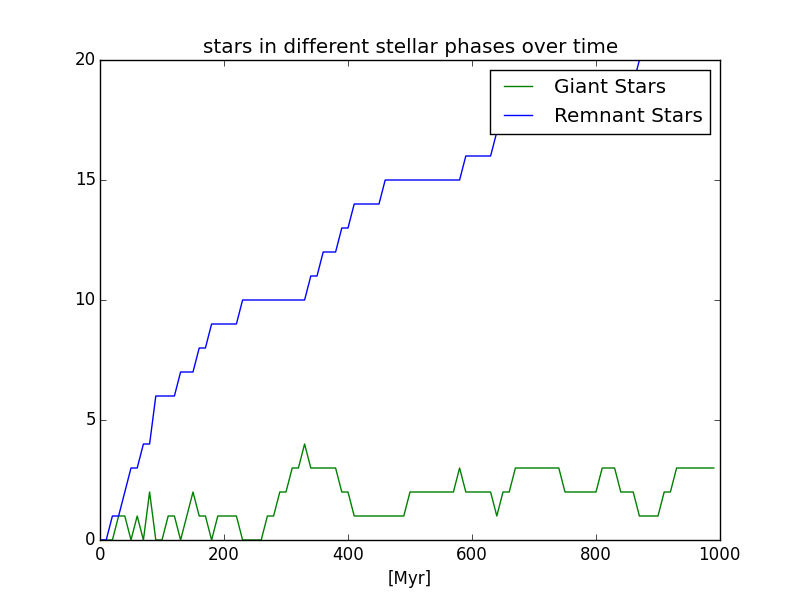
\includegraphics[width=\hsize]{img/stellar_phases_counts_without_main_sequence.png}
%     \caption{Stars in two stellar evolution categories over time (excluding main sequence stars).}\label{fig:phases_without_ms}
% \end{figure}

\section{Comments on initial code}


.... from AMUSE docmumentation: ``The bridgesys is flexible but care should be taken in order to obtain valid results. For one thing, there is no restriction or check on the validity of the assumption of well seperated dynamics: for example any system could be split up and put together in bridge, but if the timestep is chosen to be larger than the timestep criterion of the code, the integration will show errors.'' ....

The code contains both an N-body code (gravity) and an SPH code (hydro) but no call to evolve model
for either code. Where is evolve model called for these codes, and with which time interval is it called?

How is the gravitational force of the gas on the cluster calculated? And of the cluster on the gas?
What errors could this introduce? How could these be solved?

What is the mass of a 'star' in the star cluster. What is the mass of a 'gas' particle in the GMC. Is
this a problem and why?

What is the smoothing length of the SPH kernel function? What does that mean?

What is the u parameter on the gas particles? How does it aect the simulation?

Explain what happens with the orbital parameters calculated in put in orbit if you set v inf = 0 and
why?

Explain in detail what the call channels.copy() does.

Why did we choose to make the SPH particles look bigger and partially transparent?

Copy and rewrite the movie code to only produce a single frame of this movie (as pdf).

\section{Multiple GMC's}

How does the computation time scale with the number of GMC's, assuming that each GMC has the
same initial mass and number of particles.

The impact parameters (d and v1) between the star cluster and the rst GMC are easy to choose.
Discuss dierent methods to choose the impact parameters between the star cluster and the later
clusters, what is the main challenge here?

\section{Discussion}\label{sec:discussion}

\section{Conclusions}\label{sec:conclusions}
\begin{enumerate}
    \item
    \item
    \item
    \item
\end{enumerate}


\begin{acknowledgements}
The authors are grateful for the help of their supervisors Edwin van der Helm, MSc and Prof. dr. S.F. Portegies Zwart. \\

This research has made use of NASA's Astrophysics Data System.
\end{acknowledgements}


%-------------------------------------------------------------------

\bibliographystyle{aa}
%\setlength{\bibsep}{0pt} % Remove whitespace in bibliography.
\bibliography{CA_Hydro_TLRH_s1603221_SS_s1617451_report_aa}
\end{document}
